% !TEX root = coatli.tex

\chapter{The Huitzi $f/20$ Imager}

The Huitzi $f/20$ imager was installed on the COATLI telescope in December 2022. The imager is named for the mexica god \href{https://en.wikipedia.org/wiki/Huītzilōpōchtli}{Huītzilōpōchtli}, the son of the goddess Coatlicue.

Earlier, the “Interim Imager” and “Huitzi $f/8$ Imager” were installed on the telescope. For historical reference, these are described in Appendices~\ref{appendix:interim-imager} and \ref{appendix:instrument-huitzi-f8}.

\section{Overview}

\begin{figure}
\begin{center}
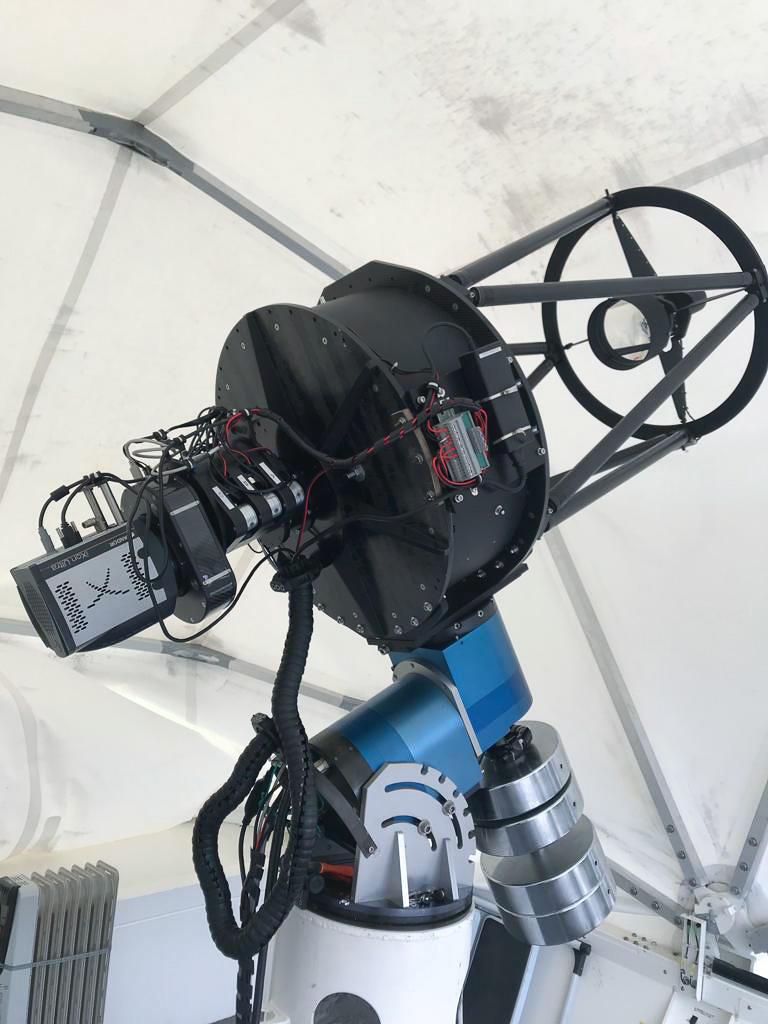
\includegraphics[width=0.7\linewidth]{figures/huitzi-on-telescope.jpg}
\medskip
\caption{The Huitzi $f/20$ imager on the COATLI telescope.}
\label{figure:huitzi-on-coatli}
\end{center}
\end{figure}

Figure~\ref{figure:huitzi-on-coatli} shows the Huitzi $f/20$ imager on the telescope.

The imager uses a 150 mm diverging lens to convert the $f/8$ beam of the telescope into an $f/20$ beam. This beam is then imaged an Andor iXon electron-multiplying CCD detector with $1024\times1024$ pixels with a pixel scale of 0.27 arcsec and a field of 4.6 arcmin. The detector can be read through either a conventional amplifier or the electron-multiplying amplifier at a variety of speeds.

The imager has three Finger Lakes Instruments filter wheels. Currently, the following filters can be provided:

\begin{itemize}
\item open: Completely open.
\item dark: Completely blocked.
\item $grizy$: Filters similar to the Pan-STARRS equivalents. Note, however, that while the filters are similar, the CCD is not deep-depleted and so the bandpasses are somewhat different.
\item $w$: A filter that combines the $r$ and $i$ bands. Note that this is different to the Pan-STARRS $w$ which includes the $g$ band too. It is mainly intended for sensitive imaging of GRBs.
\item $BVRI$: Johnson-Cousins filters according to the Bessell formulation.
\item $\Is$: The $I$ filter with a sharp red cutoff at 900 nm. This is intended to better match the bandpass of the original Cousins $I$ photomety. The blue edge is the same as the Bessell formulation, but the red edge is defined by a 900 nm short-pass filter to simulate the red edge of a GaAs tube. The Bessell (1990) and Bessell \& Murphy (2012) bandpasses fall at about 900 nm.
\item 470/10, 515/10, and 640/10: Nebular continuum filters.
\item 501/8, 656/3, 656/8: Nebular line filters.
\end{itemize}

Some of these filters are constructed from combinations of filters in different wheels, as described in more detail below.

The detector is mounted on Optec Gemini focuser/rotator, which allows up to 12.7 mm of motion of the detector with respect to the lens.

\section{Optics}

\begin{figure}
\resizebox{\columnwidth}{!}{
\begin{tikzpicture}
\draw[dashed](-10,0) -- (12,0);
\draw(-8,+2) -- (-4,+1);
\draw(-8,-2) -- (-4,-1);
\draw[dotted](-4,+1) -- (0,0) -- (-4,-1);
\draw[>-<] (-4,-2) -- (-4,+2);
\draw (-4,+1) -- (10,0) -- (-4,-1);
\draw (-4,-2.5) node {$S$};
\draw (0,-2.5) node {$A$};
\draw (10,-2.5) node {$A’$};
\end{tikzpicture}
}
\medskip
\caption{Schematic of the Optical Design}
\label{figure:optical-design}
\end{figure}

The effect of the negative lens is shown schematically in Figure~\ref{figure:optical-design}. $A$ is the position of the telescope focus without the lens. $S$ is the position of the lens. $A'$ is the position of the telescope focus with the lens. 
The magnification $m$ is given by
$$
	m = SA'/SA,
$$
in which $SA'$ and $SA$ are optical distances.
If the focal length of the lens is $F$, then Gauss’ equation gives the relation between $SA$ and $SA’$ as:
$$
	1/F = 1/SA' - 1/SA.
$$
We then solve to find:
$$
	m = 1 - SA'/F
$$
and
$$
	SA' = - (m - 1) F.
$$
We can see the approximate dimensions of the system by ignoring chromatic aberration and taking $F = -150$ mm. Then, if we choose $SA = 90$ mm we have $SA' = 225$ mm and $m = 2.5$. Since the focal ratio of the telescope is $f/8$, this magnification gives a focal ratio of $f/20$.

\begin{figure}
\begin{center}
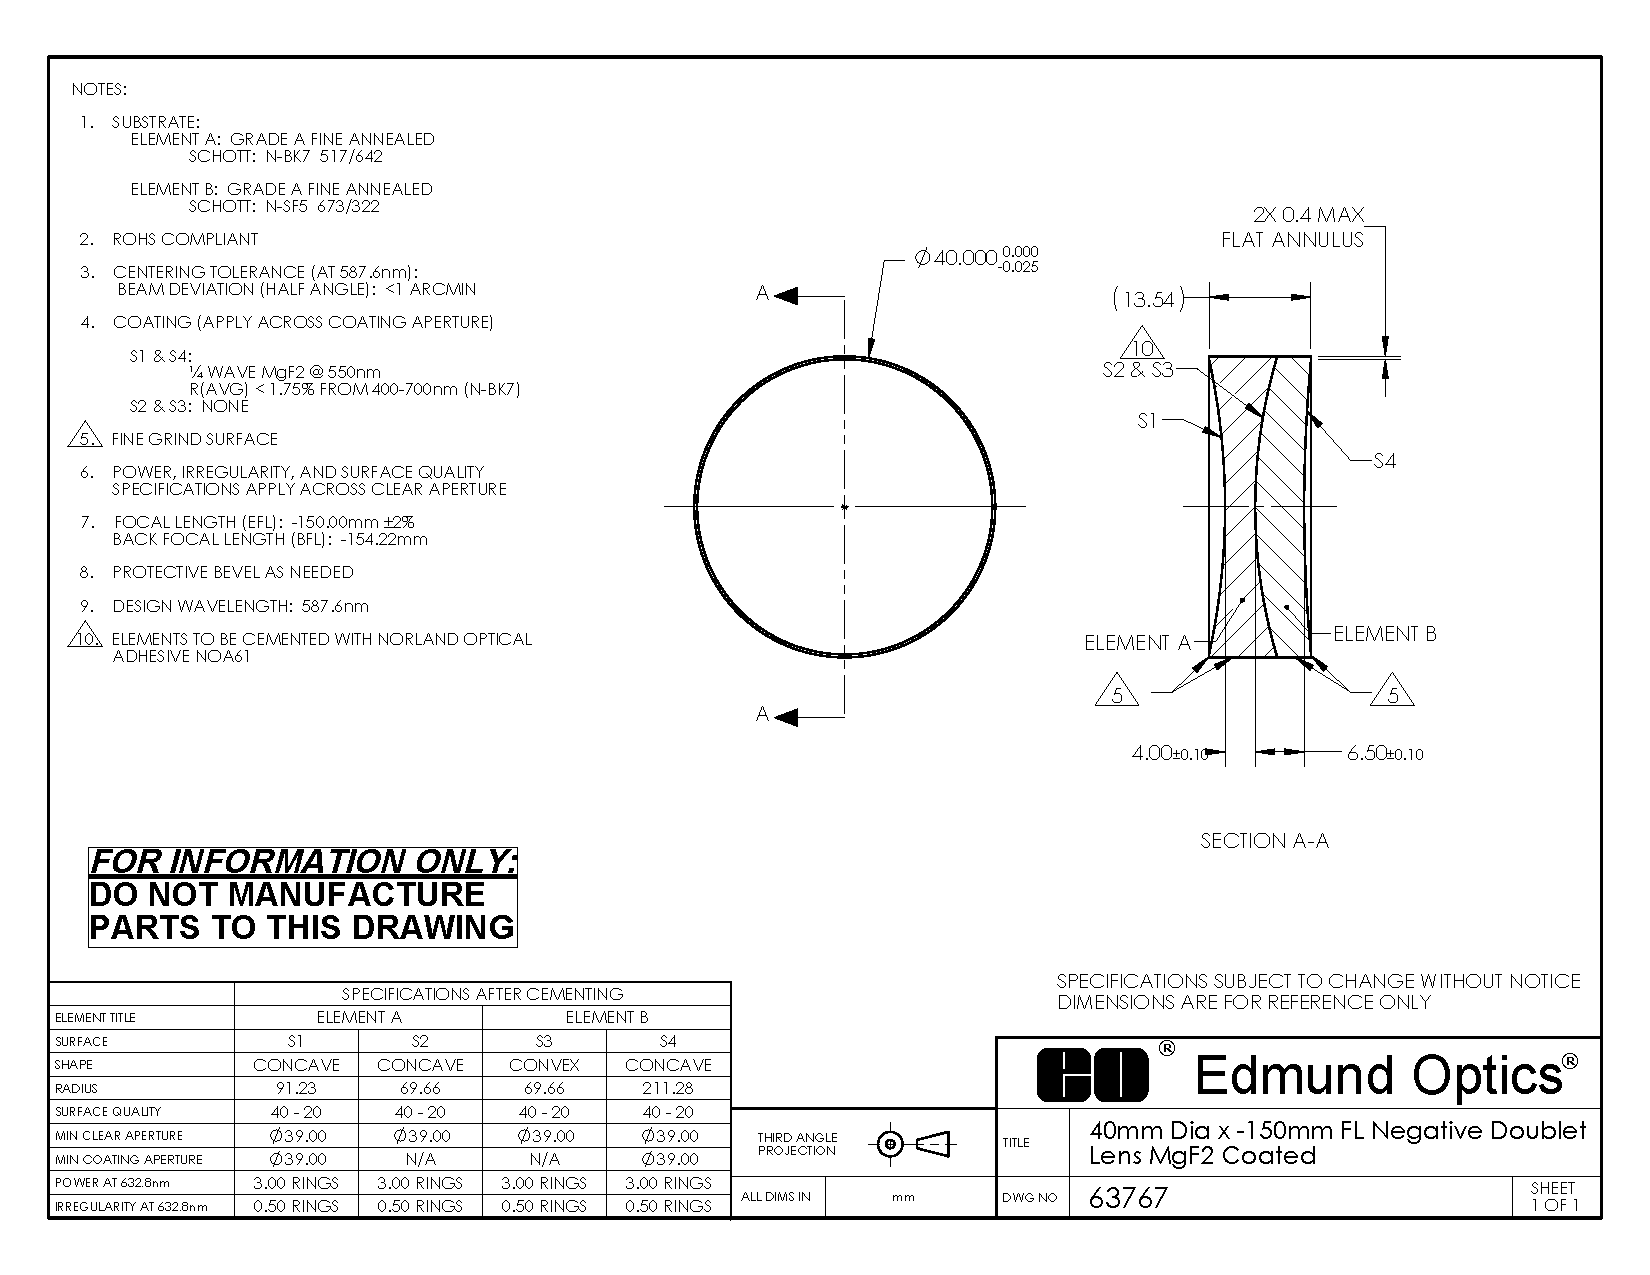
\includegraphics[width=0.8\linewidth]{figures/huitzi-lens-design.pdf}
\medskip
\caption{The lens design.}
\label{figure:huitzi-lens-design}
\end{center}
\end{figure}

The actual lens is Edmund Optics part \#63-767, whose design is shown in Figure~\ref{figure:huitzi-lens-design}. It has a design effective focal length of $-150$ mm at 587.6 nm. It is nominally 40 mm in diameter and 13.54 mm thick at the edge. The precise optical and mechanical prescriptions of are given in the files “\verb|zmax_63767.ZMX|”and “\verb|step_63767.STP|” supplied by Edmund Optics. The lens is used with the convergent element B uppermost (towards the telescope). That is surface S4 is uppermost (towards the telescope) and surface S1 is lowermost (towards the detector). If it is inverted, the system will suffer significant spherical aberration.

The lens is an achromatic doublet, so its focal length varies with wavelength. This has two effects. First, the different focal length between bands requires us to refocus for each filter. In theory, we could adjust both the secondary and the focuser to achieve focus while holding the magnification constant. In practice, we simply adjust the focuser to maintain focus and let the magnification vary slightly. (The focuser is also used to compensate for the different optical thicknesses of the filters.) Second, chromatic aberration within the $g$ and $B$ bands limits their image quality.

The lens has a $\lambda/4$ MgF$_2$ coating on both surfaces.

The lens also serves as a window to prevent ingress of dust and insects.

\section{Bibliography}

\begin{flushleft}
\begin{itemize}
\item “\href{bibliography/huitzi/andor-ixon-ultra-888-data-sheet.pdf}{Andor iXon Ultra 888 Data Sheet}”, Andor, May 2014.
\item “\href{bibliography/huitzi/andor-ixon-ultra-888-hardware-guide.pdf}{Andor iXon Ultra \& Life 888 Hardware Guide}”, Andor, Version 1.8 of 30 September 2019.
\item Bessell, M.S., 1990, PASP, 102, 1181: “$UBVRI$ Passbands”.
\item Bessell, M., \& Murphy, S., 2012,  PASP, 124, 140: “Spectrophotometric Libraries, Revised Photonic Passbands, and Zero Points for UBVRI, Hipparcos, and Tycho Photometry”.
\item “\href{bibliography/huitzi/e2v-ccd201-20-datasheet.pdf}{CCD201-20 Datasheet}”, Teledyne e2v, Version 7 of August 2019.
\end{itemize}
\end{flushleft}


